\documentclass{article}
\usepackage{siunitx} 
\usepackage{graphicx}
\usepackage{natbib}
\usepackage{amsmath} 

\setlength\parindent{0pt}

\renewcommand{\labelenumi}{\alph{enumi}.}

%\usepackage{times} 

%----------------------------------------------------------------------------------------
%	DOCUMENT INFORMATION
%----------------------------------------------------------------------------------------

\title{Práctica 5 \\ Programación Concurrente y de Tiempo Real \\Universidad de Cádiz} % Title

\author{Alejandro Serrano Fernández} % Author name

\date{\today} % Date for the report

\begin{document}

\maketitle % Insert the title, author and date


%----------------------------------------------------------------------------------------
%	SECTION 1
%----------------------------------------------------------------------------------------

\section{Primos Paralelos}
Para calcular el tiempo que tarda mi computadora en realizar el cálculo, cabe destacar que he utilizado un tamaño de entrada de 10000000 números. Los siguientes datos han sido obtenidos a través de un portátil equipado con un i7-7700hq de 4 núcleos y 8 threads. Como podemos observar para este problema, a medida que aumentamos el número de hilos el tiempo de ejecución disminuye, presentando así una mejora con respecto a la versión secuencial de este problema.
\hfill \break
\begin{center}
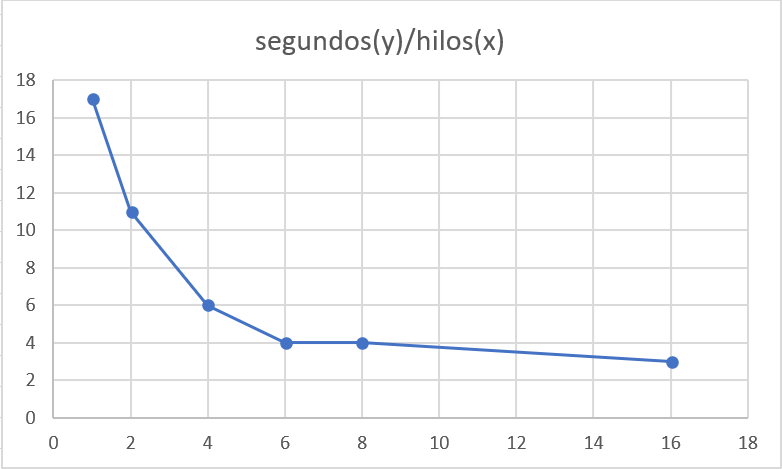
\includegraphics[scale=0.5]{grafica-ejercicio1-primos-tiempo-hilos.png}
\end{center}
\hfill \break
Destacar también, que al obtener mejores resultados, el Speedup para este problema aumenta notablemente. Esto significa que para mayor número de hilos, obtenemos una mayor aceleración del cálculo.
\hfill \break
\begin{center}
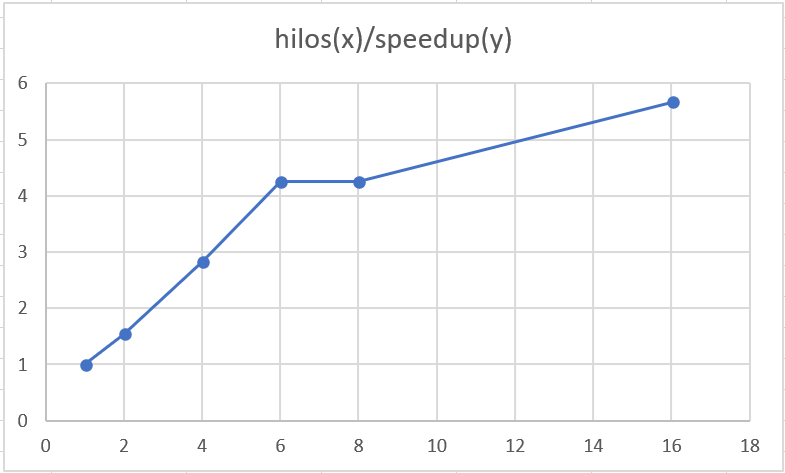
\includegraphics[scale=0.5]{grafica-ejercicio1-primos-hilos-speedup.png}
\end{center}

\section{Volcado Red}
Para este problema, utilizo la misma computadora que en el problema anterior. Como se puede observar en el gráfico, hay una notable mejora entre los Cb 0.2 y 0.8, aunque para un cb intermedio he podido observar que los resultados son muy parecidos y dispares, pues el tiempo también depende de la latencia de la red, la cual puede variar dependiendo de múltiples factores (lugar en el que se ubica el servidor, capacidad de cómputo del servidor web, congestión de la red...), por lo que podemos concluir que estos resultados no son recomendados para determinar si hay una mejora. Los resultados han sido los siguientes (x = tiempo, y = Cb):
\hfill \break
\begin{center}
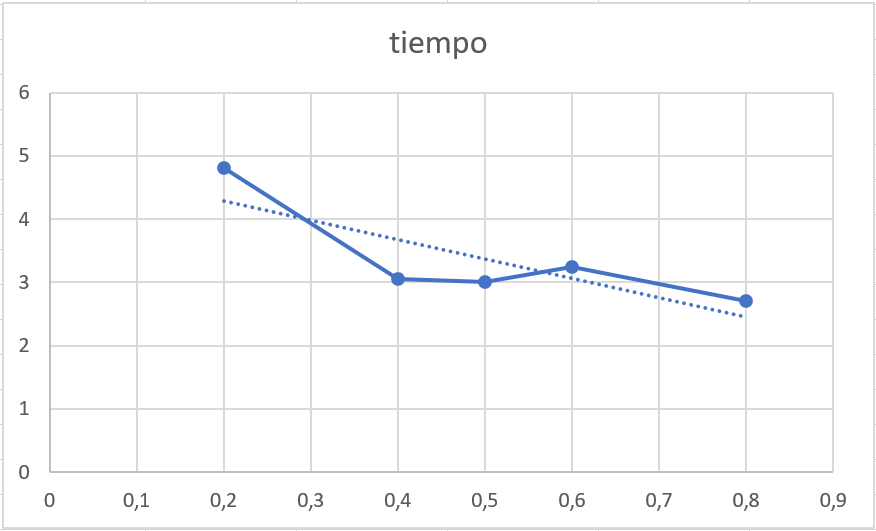
\includegraphics[scale=0.45]{grafico-ejercicio1-red-tiempo-cb.png}

\end{center}

\end{document}




